\documentclass[12pt]{article}
\usepackage[utf8]{inputenc} % utf8 support

% === Document Layout ===
\usepackage[hmargin=1in,vmargin=1in]{geometry}
\usepackage{indentfirst}
\usepackage{lipsum}
\usepackage{url}
\usepackage[colorlinks,linkcolor=red!50!black,citecolor=blue!50!black,urlcolor=blue!50!black]{hyperref}
\usepackage{amsmath}
\usepackage{pdfpages}
\usepackage{physics}
\usepackage{xcolor}
\usepackage{graphicx}
\usepackage{mathtools} % for the coloneq command
\usepackage{xparse}
\usepackage{ifthen} % For checking optional parameters
\usepackage{enumerate}
\usepackage{mathrsfs} % For \mathscr font
\usepackage{amsthm} % The AMS theorems package
\usepackage{amsthm}
\usepackage{tabularx}

% amsthm
\newtheorem{theorem}{Theorem}[section]
\newtheorem{corollary}{Corollary}[theorem]
\newtheorem{lemma}[theorem]{Lemma}
\theoremstyle{definition}
\newtheorem{definition}{Definition}[section]
\theoremstyle{remark}
\newtheorem*{remark}{Remark}

\usepackage{amsfonts}
\usepackage{indentfirst}
\usepackage{pgfplots}
\usepackage{tikz}
\usetikzlibrary{
    calc,
    arrows,
    shapes.geometric,
    intersections,
    pgfplots.fillbetween,
    decorations.pathreplacing,
    decorations.markings
}
\tikzset{every picture/.style={baseline={([yshift=-0.3em]current bounding box.center)}}}
\tikzset{
    % style to apply some styles to each segment of a path
    on each segment/.style={
        decorate,
        decoration={
            show path construction,
            moveto code={},
            lineto code={
                \path [#1]
                (\tikzinputsegmentfirst) -- (\tikzinputsegmentlast);
            },
            curveto code={
                \path [#1] (\tikzinputsegmentfirst)
                .. controls
                (\tikzinputsegmentsupporta) and (\tikzinputsegmentsupportb)
                ..
                (\tikzinputsegmentlast);
            },
            closepath code={
                \path [#1]
                (\tikzinputsegmentfirst) -- (\tikzinputsegmentlast);
            },
        },
    },
    % style to add short perpendicular bar midway along a path
    bar/.style={
        postaction={
            decorate,
            decoration={
                markings,
                mark=at position .5 with {\arrow{|}}
            }
        }
    }
}

\DeclareMathOperator{\id}{id}
\newcommand{\opcat}{\mathrm{op}}
\DeclareMathOperator{\Hom}{Hom}
\DeclareMathOperator{\cod}{cod}
\DeclareMathOperator{\dom}{dom}

% === Bibliography ===
\usepackage[
    backend=biber,
    style=alphabetic,
]{biblatex}
\addbibresource{references.bib}

\begin{document}
\begin{center}
    \large{\textbf{Towards a General Theory of Elimination (and Optimization?)}} \\
    \normalsize{TC Fraser, Tobias Fritz} \\
    \normalsize{Perimeter Institute for Theoretical Physics} \\
    \normalsize{June 7th, 2019}
\end{center}

\newcommand{\catA}{\mathscr{A}}
\newcommand{\catB}{\mathscr{B}}
\newcommand{\catC}{\mathscr{C}}
\newcommand{\catD}{\mathscr{D}}
\newcommand{\catE}{\mathscr{E}}

\section{Preliminaries}

\subsection{Hom-Functors}
For a locally small category $\catC$, the hom-functor of $\catC$ is a functor $\Hom_{\catC} : \catC^{\opcat} \times \catC \to \mathbf{Set}$ constructed in the following manner. Given objects $a,b,c,\ldots \in \catC_0$ of $\catC$, the hom-functor $\Hom_{\catC}$ maps a pair of objects $(a,b) \in (\catC^\opcat \times \catC)_0 = \catC_0 \times \catC_0 = \catC_0^2$ into the set\footnote{The collection of morphisms of type $a \to b$ forms a set because $\catC$ is locally small.} of morphisms $\catC_1$ of $\catC$ with source $a$ and target $b$. Therefore, $\Hom_{\catC}(a,b)$ is the set of morphisms in $\catC$ of type $a \to b$. Given morphisms $g^{\opcat} \in \Hom_{\catC^{\opcat}}(a,c)$ and $h \in \Hom_{\catC}(b,d)$, the hom-functor $\Hom_{\catC}$ constructs a function
\[ \Hom_{\catC}(g^{\opcat}, h) : \Hom_{\catC}(a,b) \to \Hom_{\catC}(c,d) \]
which takes a morphism $f : a \to b \in \Hom_{\catC}(a,b)$ and produces the morphism $h \circ f \circ g : c \to d \in \Hom_{\catC}(c,d)$. Graphically,
\[
    \Hom_{\catC}(g^{\opcat}, h)
    \left(
    \begin{tikzpicture}
        \draw (0,0) node(a){$a$};
        \draw (1,0) node(b){$b$};
        \draw[->] (a) to node[above, midway]{$f$} (b);
    \end{tikzpicture}
    \right)
    =
    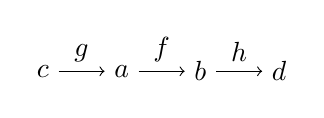
\begin{tikzpicture}
        \draw (0,0) node(c){$c$};
        \draw (1,0) node(a){$a$};
        \draw (2,0) node(b){$b$};
        \draw (3,0) node(d){$d$};
        \draw[->] (c) to node[above, midway]{$g$} (a);
        \draw[->] (a) to node[above, midway]{$f$} (b);
        \draw[->] (b) to node[above, midway]{$h$} (d);
    \end{tikzpicture}
\]

\subsection{Adjoint Functors}
Given two categories $\mathscr{C}$ and $\mathscr{D}$, a pair of functors $L : \mathscr C \to \mathscr D, R : \mathscr D \to \mathscr C$ are called an \textit{adjoint pair}, denoted $L \dashv R$ or
\[
    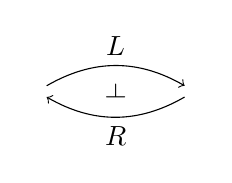
\begin{tikzpicture}
        \draw (0,0) node(c){$\catC$};
        \draw (2,0) node(d){$\catD$};
        \draw[->] (c) to[bend left] node[above, midway]{$L$} (d);
        \draw[->] (d) to[bend left] node[below, midway]{$R$} (c);
        \draw (1,0) node[rotate=-90]{$\dashv$};
    \end{tikzpicture}
\]
if there exists a natural isomorphism $\alpha$ between the following pair of hom-functors of type $\mathscr C^{\opcat} \times \mathscr D \to \mathbf{Set}$:
\[ \Hom_{\mathscr D}(L^{\opcat}(-), -) \stackrel{\alpha}{\simeq} \Hom_{\mathscr C}(-, R(-)) \]
This relationship can be depicted graphically as $2$-cell (and its inverse) in $\mathbf{Cat}$,
\[
    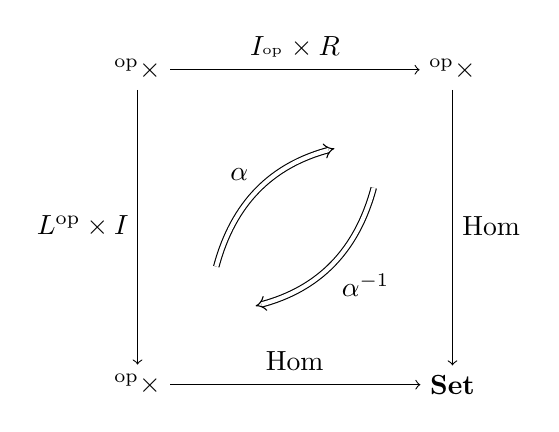
\begin{tikzpicture}
        \draw (0,4) node(tl){$\catC^\opcat \times \catD$};
        \draw (4,4) node(tr){$\catC^\opcat \times \catC$};

        \draw (0,0) node(bl){$\catD^{\opcat} \times \catD$};
        \draw (4,0) node(br){$\mathbf{Set}$};
        \draw[->] (tl) to node[midway, above]{$I_{\catC^{\opcat}} \times R$} (tr);
        \draw[->] (bl) to node[midway, above]{$\Hom_{\catD}$} (br);
        \draw[->] (tl) to node[midway, left]{$L^{\opcat} \times I_{\catD}$} (bl);
        \draw[->] (tr) to node[midway, right]{$\Hom_{\catC}$} (br);

        \draw[double equal sign distance, -implies] (1,1.5) to[bend left] node[above left]{$\alpha$} (2.5,3);
        \draw[double equal sign distance, -implies] (3,2.5) to[bend left] node[below right]{$\alpha^{-1}$} (1.5,1);
    \end{tikzpicture}
\]
Concretely, the naturality of $\alpha$ means that for every morphism $(f^{\opcat} : b \to a, g : c \to d) \in (\catC^{\opcat} \times \catD)_1$ the components $\alpha_{(b,c)}$ and $\alpha_{(a,d)}$ of $\alpha$ make the following square commute:
\[
    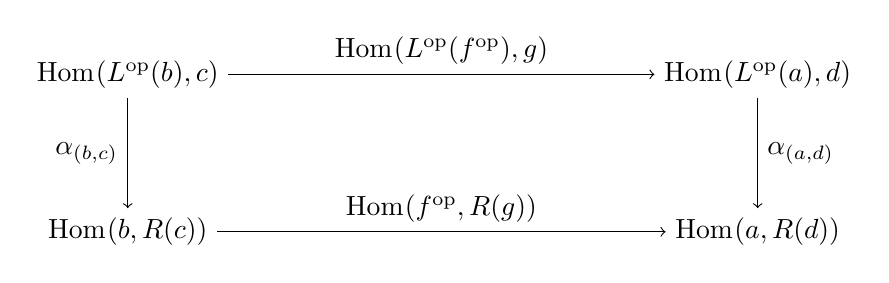
\begin{tikzpicture}
        \draw (0,2) node(tl){$\Hom_{\catD}(L^{\opcat}(b), c)$};
        \draw (8,2) node(tr){$\Hom_{\catD}(L^{\opcat}(a), d)$};
        \draw[->] (tl) to node[midway, above]{$\Hom_{\catD}(L^{\opcat}(f^{\opcat}), g)$} (tr);

        \draw (0,0) node(bl){$\Hom_{\catC}(b, R(c))$};
        \draw (8,0) node(br){$\Hom_{\catC}(a, R(d))$};
        \draw[->] (bl) to node[midway, above]{$\Hom_{\catC}(f^{\opcat}, R(g))$} (br);

        \draw[->] (tl) to node[midway, left]{$\alpha_{(b,c)}$} (bl);
        \draw[->] (tr) to node[midway, right]{$\alpha_{(a,d)}$} (br);
    \end{tikzpicture}
\]

\subsection{Beck-Chevalley Conditions}

The Beck-Chevalley Conditions are conditions that may or may not be satisfied by a quadruplet of functors $F,H,G,K$ which form a natural isomorphism $\alpha : K F \Rightarrow H G$ square:

\[
    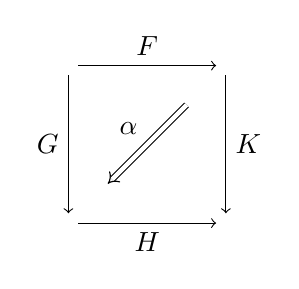
\begin{tikzpicture}
        \draw (-1,+1) node(tl){$\catA$};
        \draw (+1,+1) node(tr){$\catB$};
        \draw (-1,-1) node(bl){$\catC$};
        \draw (+1,-1) node(br){$\catD$};

        \draw[->] (tl) to node[above]{$F$} (tr);
        \draw[->] (tl) to node[left ]{$G$} (bl);
        \draw[->] (bl) to node[below]{$H$} (br);
        \draw[->] (tr) to node[right]{$K$} (br);

        \draw[double equal sign distance, -implies] (+0.5,+0.5) to node[above left]{$\alpha$} (-0.5,-0.5);
    \end{tikzpicture}
\]
To define the \textit{left} Beck-Chevalley condition, one needs functors $F_L : \catB \to \catA$ and $H_L : \catD \to \catA$ which are respectively left adjoint functors to $F$ and $H$, 

\[
    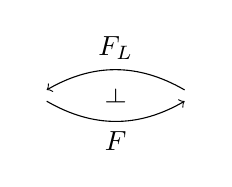
\begin{tikzpicture}
        \draw (-1,+1) node(tl){$\catA$};
        \draw (+1,+1) node(tr){$\catB$};

        \draw[->] (tl) to[bend right] node[below]{$F$} (tr);
        \draw[->] (tr) to[bend right] node[above]{$F_L$} (tl);
        \draw (0,+1) node[rotate=-90]{$\dashv$};
    \end{tikzpicture}
    ,
    \qquad 
    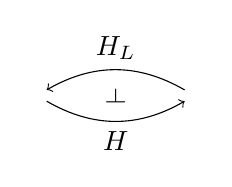
\begin{tikzpicture}
        \draw (-1,-1) node(bl){$\catC$};
        \draw (+1,-1) node(br){$\catD$};

        \draw[->] (bl) to[bend right] node[below]{$H$} (br);
        \draw[->] (br) to[bend right] node[above]{$H_L$} (bl);
        \draw (0,-1) node[rotate=-90]{$\dashv$};
    \end{tikzpicture}
    .
\]
Using these left adjoint functors, it becomes possible to construct a natural transformation $\beta : KH_L \Rightarrow GF_L$ from $\alpha$\footnote{The natural transformations $\alpha$ and $\beta$ are known as \textit{mates} or \textit{conjugates}.}. Graphically, $\beta$ can be identified as the outer cell of the following diagram:
\[
    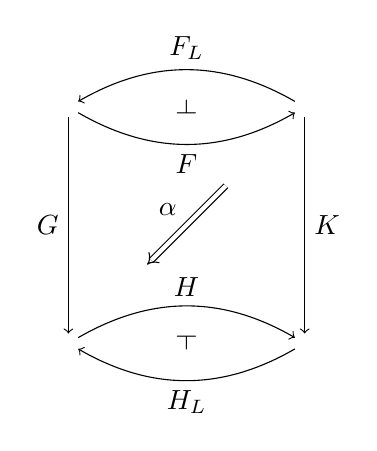
\begin{tikzpicture}
        \draw (-1.5,+1.5) node(tl){$\catA$};
        \draw (+1.5,+1.5) node(tr){$\catB$};
        \draw (-1.5,-1.5) node(bl){$\catC$};
        \draw (+1.5,-1.5) node(br){$\catD$};

        \draw[->] (tl) to[bend right] node[below]{$F$} (tr);
        \draw[->] (tr) to[bend right] node[above]{$F_L$} (tl);
        \draw (0,+1.5) node[rotate=-90]{$\dashv$};
        \draw[->] (tl) to node[left ]{$G$} (bl);
        \draw[->] (bl) to[bend left ] node[above]{$H$} (br);
        \draw[->] (br) to[bend left ] node[below]{$H_L$} (bl);
        \draw (0,-1.5) node[rotate=+90]{$\dashv$};
        \draw[->] (tr) to node[right]{$K$} (br);

        \draw[double equal sign distance, -implies] (+0.5,+0.5) to node[above left]{$\alpha$} (-0.5,-0.5);
    \end{tikzpicture},
    \qquad
    \text{i.e.}
    \qquad
    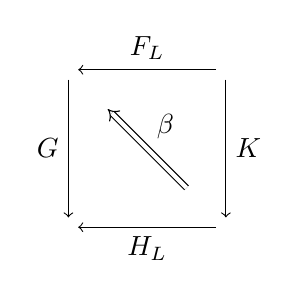
\begin{tikzpicture}
        \draw (-1,+1) node(tl){$\catA$};
        \draw (+1,+1) node(tr){$\catB$};
        \draw (-1,-1) node(bl){$\catC$};
        \draw (+1,-1) node(br){$\catD$};

        \draw[->] (tr) to node[above]{$F_L$} (tl);
        \draw[->] (tl) to node[left ]{$G$} (bl);
        \draw[->] (br) to node[below]{$H_L$} (bl);
        \draw[->] (tr) to node[right]{$K$} (br);

        \draw[double equal sign distance, -implies] (+0.5,-0.5) to node[above right]{$\beta$} (-0.5,+0.5);
    \end{tikzpicture}.
\]
Although the natural transformation $\alpha$ is assumed to be a natural isomorphism, the natural transformation $\beta$ need not be; if $\beta$ happens to be a natural isomorphism, then we say that the original square satisfies the \textit{left} Beck-Chevalley condition\footnote{Are the left adjoints $F_L, H_L$ unique? If not, it might be better to say the original square satifies the left Beck-Chevalley condition with respect to $F_L, H_L$.}. The \textit{right} Beck-Chevalley condition is defined analogously with functors $F_R, H_R$ which are respectively right adjoints $F \dashv F_R$ and $H \dashv H_R$.

\subsection{Cartesian Morphisms}

A morphism $\phi : e' \to e$ in $\catE$ is \textit{cartesian} with respect to a functor $P : \catE \to \catB$ if for every $\psi : e'' \to e$ in $\catE$ and for every $g : P(e'') \to P(e')$ such that $ P(\phi) \circ_{\catB} g = P(\psi)$ (i.e. such that the second diagram commutes), there exists a unique morphism $\sigma : e'' \to e'$ in $\catE$ such that $\phi \circ_{\catE} \sigma = \psi$ (i.e. such that the first diagram commutes):\footnote{The definition and treatment of Cartesian morphisms found in the \textit{Reformulations} section of \url{https://ncatlab.org/nlab/show/Cartesian+morphism\#CartInOrdCatReformulation} is probably better suited here.}

\[
    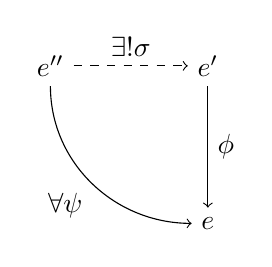
\begin{tikzpicture}
        \draw (-1,+1) node(tl){$e''$};
        \draw (+1,+1) node(tr){$e'$};
        \draw (+1,-1) node(br){$e$};

        \draw[dashed, ->] (tl) to node[above]{$\exists!\sigma$} (tr);
        \draw[->] (tl) to[out=-90, in=180] node[below left]{$\forall\psi$} (br);
        \draw[->] (tr) to node[right]{$\phi$} (br);
    \end{tikzpicture}
    \qquad
    \stackrel{P}{\mapsto}
    \qquad
    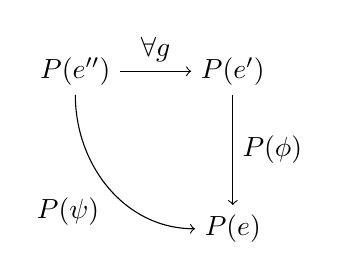
\begin{tikzpicture}
        \draw (-1,+1) node(tl){$P(e'')$};
        \draw (+1,+1) node(tr){$P(e')$};
        \draw (+1,-1) node(br){$P(e)$};

        \draw[->] (tl) to node[above]{$\forall g$} (tr);
        \draw[->] (tl) to[out=-90, in=180] node[below left]{$P(\psi)$} (br);
        \draw[->] (tr) to node[right]{$P(\phi)$} (br);
    \end{tikzpicture}
\]
\subsection{Grothendieck Fibrations}

A functor $P : \catE \to \catB$ is a \textit{Grothendieck fibration} if it satisfies the following ``lifting'' property that for every morphism $f : b \to P(e)$ of $\catB$ (i.e. if the codomain of $f$ is contained in the image of $P$), there exists a \textit{cartesian} morphism $\phi : e' \to e$ of $\catE$ in the fibre category $\catE_{P(e)}$ (i.e. $P(\phi) = f$).

\subsection{The Equivalence of Pseudofunctors and Fibrations}

Given a functor $P : \catE \to \catB$ which is also a Grothendieck fibration equipped with a cleavage (i.e. a choice of cartesian morphism $\phi \in \Hom_{\catE}(e', e)$ for each $f \in \Hom_{\catB}(a,P(e))$ such that $P(\phi) = f$), it is possible to construct a pseudofunctor (read weak $2$-functor between weak $2$-categories) $\pi : \catB^{\opcat} \to \mathbf{Cat}$. In particular, each object $b \in \catB_0$ is mapped to the \textit{sub-category} $\pi(b) = \catE_b$ of $\catE$ whose objects are those which map to $b$ under $P$ and whose morphism are those which map to $\id_{b}$ under $P$; $\catE_b$ is the fibre category over $b$ with respect to $P$. For each morphism $f \in \Hom_{\catB}(a,b)$ in $\catB$, the pseudofunctor $\pi$ maps $f^{\opcat} : b \to a$ onto a functor $\pi(f^{\opcat}) = f^{\ast} : \catE_{b} \to \catE_{a}$ which is defined accordingly:
\[
    \begin{tikzpicture}
        \begin{scope}[shift={(-4.5,0)}]
            \draw (-3,+3) rectangle (+3,-3) node[above left]{$\catE$};
            \begin{scope}[shift={(-1,+2.5)}]
                \draw (0,0) rectangle (+3.5,-2) node[above left](catEa){$\catE_a$};
                \draw (+0.5, -0.8) node(e2){$e'$};
                \draw (+2, -0.8) node(e4){$e'''$};
                \draw[->] (e2) to node[above]{$\psi'$} (e4);
            \end{scope}
            \begin{scope}[shift={(-2,-0.5)}]
                \draw (0,0) rectangle (+3.5,-2) node[above left](catEb){$\catE_b$};
                \draw (+0.5, -1.2) node(e1){$e$};
                \draw (+2, -1.2) node(e3){$e''$};
                \draw[->] (e1) to node[below]{$\psi$} (e3);
            \end{scope}
            \draw[white, line width=2mm] (e2) to[out=-90,in=+90] (e1);
            \draw[white, line width=2mm] (e4) to[out=-90,in=+90] (e3);
            \draw[->] (e2) to[out=-90,in=+90] node[left ]{$\phi$} (e1);
            \draw[->] (e4) to[out=-90,in=+90] node[right]{$\phi'$} (e3);
            \draw[->] (catEb) to[out=0,in=-90] node[right]{$f^{\ast}$} (catEa);
        \end{scope}
        \begin{scope}[shift={(+1.5,+1)}]
            \draw (0,0) rectangle (+2,-2) node[above left]{$\catB$};
            \draw (+1.2, -0.3) node(a){$a$};
            \draw (+0.8,-1.6) node(b){$b$};
            \draw[->] (a) to[out=-90,in=+90] node[right]{$f$} (b);
        \end{scope}
        \draw[->] (-1,+0.5) to[bend left ] node[above]{$P$} (+1, 0.5);
        \draw[<-] (-1,-0.5) to[bend right] node[below]{$P^{\leftarrow}$} (+1, -0.5);
    \end{tikzpicture}
\]
Given an object $e \in (\catE_b)_0$, the functor $f^{\ast}$ finds the unique cartesian morphism $\phi \in \Hom_{\catE}(e',e)$ as specified by the cleavage and assigns $f^{\ast}(e) = e'$. Next, given a morphism $\psi \in \Hom_{\catE_{b}}(e, e'')$, the functor $f^{\ast}$ first finds the unique cartesian morphisms $\phi \in \Hom_{\catE}(e', e)$ and $\phi' \in \Hom_{\catE}(e''', e'')$. Then, because $g = \id_a$ completes the following diagram
\[
    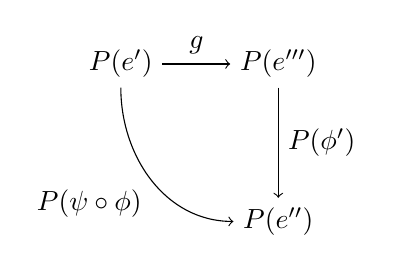
\begin{tikzpicture}
        \draw (-1,+1) node(tl){$P(e')$};
        \draw (+1,+1) node(tr){$P(e''')$};
        \draw (+1,-1) node(br){$P(e'')$};

        \draw[->] (tl) to node[above]{$g$} (tr);
        \draw[->] (tl) to[out=-90, in=180] node[below left]{$P(\psi\circ\phi)$} (br);
        \draw[->] (tr) to node[right]{$P(\phi')$} (br);
    \end{tikzpicture}
    \quad=\quad
    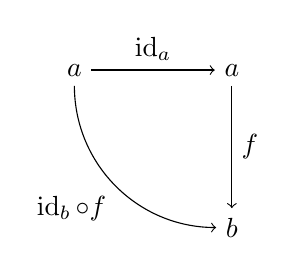
\begin{tikzpicture}
        \draw (-1,+1) node(tl){$a$};
        \draw (+1,+1) node(tr){$a$};
        \draw (+1,-1) node(br){$b$};

        \draw[->] (tl) to node[above]{$\id_{a}$} (tr);
        \draw[->] (tl) to[out=-90, in=180] node[below left]{$\id_{b} \circ f$} (br);
        \draw[->] (tr) to node[right]{$f$} (br);
    \end{tikzpicture},
\]
and because $\phi'$ is cartesian, there must exist a unique $\psi' \in \Hom_{\catE_a}(e', e''')$ such that $\psi \circ \phi = \phi' \circ \psi'$. For each $\psi \in \Hom_{\catE_b}(e, e'')$, the functor $f^{\ast}$ selects this unique morphism $f^{\ast}(\psi) = \psi'$. In summary, the pseudofunctor $\pi : \catB^{\opcat} \to \mathbf{Cat}$ induced by $P : \catE \to \catB$ is defined on objects $b \in \catB_{0}$ as $\pi(b) = \catE_{b}$ and on morphisms $f \in \catB_{1}$ as $\pi(f) = f^{\ast}$ and forms a functor \textcolor{red!50!black}{[TODO: figure out the `pseudo' part of the pseudofunctorality.]}.

\subsection{Slice and Coslice Categories}

Given a category $\catC$ and an object $c \in \catC_0$ of $\catC$, the \textit{slice category} (or \textit{over category}) $\catC/c$ is the ``stuff in $\catC$ that is on top of $c$''. Specifically, the objects of $\catC/c$ are all the morphisms $f \in \catC_1$ from $\catC$ whose codomain is $\cod(f) = c$ (alternatively you could write $(\catC/c)_0 = \Hom_{\catC}(-,c)$). A morphism of $\catC/c$ between objects $f : a \to c, g : b \to c \in (\catC/c)_0$ is a commuting triangle completed by a third morphism $h : a \to b \in \catC_1$:

\[
    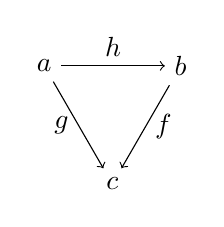
\begin{tikzpicture}
        \draw (150:1) node(tl){$a$};
        \draw ( 30:1) node(tr){$b$};
        \draw (270:1)node(bm){$c$};

        \draw[->] (tl) to node[below,left ]{$g$} (bm);
        \draw[->] (tr) to node[below,right]{$f$} (bm);

        \draw[->] (tl) to node[above]{$h$} (tr);
    \end{tikzpicture}
\]
Composition of morphisms in $\catC/c$ is induced by the composition of morphisms in $\catC$:
\[
    \left(
    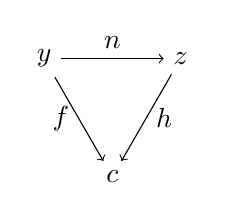
\begin{tikzpicture}
        \draw (150:1) node(tl){$y$};
        \draw ( 30:1) node(tr){$z$};
        \draw (270:1) node(bm){$c$};

        \draw[->] (tl) to node[below,left ]{$f$} (bm);
        \draw[->] (tr) to node[below,right]{$h$} (bm);

        \draw[->] (tl) to node[above]{$n$} (tr);
    \end{tikzpicture}
    \right)
    \circ_{\catC/c}
    \left(
    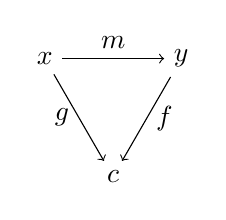
\begin{tikzpicture}
        \draw (150:1) node(tl){$x$};
        \draw ( 30:1) node(tr){$y$};
        \draw (270:1) node(bm){$c$};

        \draw[->] (tl) to node[below,left ]{$g$} (bm);
        \draw[->] (tr) to node[below,right]{$f$} (bm);

        \draw[->] (tl) to node[above]{$m$} (tr);
    \end{tikzpicture}
    \right)
    =
    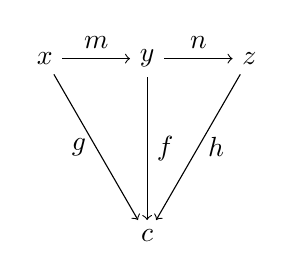
\begin{tikzpicture}
        \draw (150:1.5) node(tl){$x$};
        \draw ( 90:0.75) node(tm){$y$};
        \draw ( 30:1.5) node(tr){$z$};
        \draw (270:1.5) node(bm){$c$};

        \draw[->] (tl) to node[below,left ]{$g$} (bm);
        \draw[->] (tm) to node[right]{$f$} (bm);
        \draw[->] (tr) to node[below,right]{$h$} (bm);

        \draw[->] (tl) to node[above]{$m$} (tm);
        \draw[->] (tm) to node[above]{$n$} (tr);
    \end{tikzpicture}
\]

The assignment of an overcategory $\catC/c$ to each object $c$ can be extended to a \textit{slice functor} $\catC / (-) : \catC \to \mathbf{Cat}$ in the following sense. For objects $c \in \catC_0$, the slice functor takes $c$ to the slice category $\catC/c$; for morphisms $f : a \to b \in \catC_1$, the slice functor takes $f$ to the functor $\catC / f : \catC / a \to \catC / b$ defined graphically; for every morphism of $\catC / a$ (commuting triangle in $\catC$ over $a$), contruct the morphism of $\catC / b$ (commuting triangle in $\catC$ over $b$) as follows:
\[
    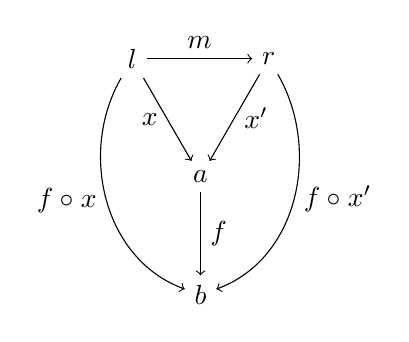
\begin{tikzpicture}
            \draw (150:1) node(tl){$l$};
            \draw ( 30:1) node(tr){$r$};
            \draw (270:1) node(bm){$a$};
            \draw (270:2.5) node(bb){$b$};

            \draw[->] (tl) to node[below,left ]{$x$}  (bm);
            \draw[->] (tr) to node[below,right]{$x'$} (bm);
            \draw[->] (tl) to[out=-120, in=+160] node[below,left ]{$f \circ_{\catC} x$}  (bb);
            \draw[->] (tr) to[out= -60, in= +20] node[below,right]{$f \circ_{\catC} x'$} (bb);
            \draw[->] (tl) to node[above]{$m$} (tr);
            \draw[->] (bm) to node[right]{$f$} (bb);
    \end{tikzpicture}
\]
where the inner triangle is a morphism of $\catC/a$ and the outer triangle is a morphism of $\catC/b$ given by the functor $\catC/f$.

Given a category $\catC$ and an object $c \in \catC_0$ of $\catC$ the \textit{coslice category} (or \textit{under category}) $c/\catC$ is the ``stuff in $\catC$ that is underneath $c$''. Specifically, the objects of $c/\catC$ are all the morphisms $f \in \catC_1$ from $\catC$ whose domain is $\dom(f) = c$ (alternatively you could write $(c/\catC)_0 = \Hom_{\catC}(c,-)$). A morphism of $c/\catC$ between objects $f : c \to a, g : c \to b \in (c/\catC)_0$ is a commuting triangle completed by a third morphism $h : a \to b \in \catC_1$:

\[
    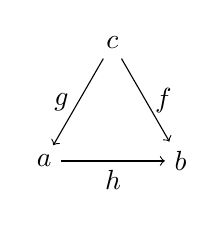
\begin{tikzpicture}
        \draw (210:1) node(tl){$a$};
        \draw (330:1) node(tr){$b$};
        \draw ( 90:1) node(bm){$c$};

        \draw[<-] (tl) to node[below,left ]{$g$} (bm);
        \draw[<-] (tr) to node[below,right]{$f$} (bm);
        \draw[->] (tl) to node[below]{$h$} (tr);
    \end{tikzpicture}
\]
Everything about coslice categories is defined as expected analogously to that of a slice categories.
\textcolor{red!50!black}{[TODO: determine how the details of the Grothendieck construction transform the slice (pseudo-)functor $\catC / (-) : \catC \to \mathbf{Cat}$ into the codomain fibration.]}
\subsection{The Pullback and Pushforward Functors}

Given a category $\catC$ and a morphism $f : a \to b \in \catC_1$, the image of $f$ under the slice functor $\catC / (-)$ produces a functor $\catC / f : \catC / a \to \catC / b$ between slice categories of $\catC$ in the ``same direction'' as $f$ \textcolor{red!50!black}{TODO: confirm that $\catC / f$ is the pushforward functor $f_{!}$ of $f \in \catC_1$.}

If the given category $\catC$ admits pullbacks, in becomes possible to define, for a morphism $f : a \to b$ a pullback functor $f^{*} : \catC / b \to \catC / a$. Given a morphism in $\catC/b$ (commuting triangle in $\catC$ with base at $b$),
\[
    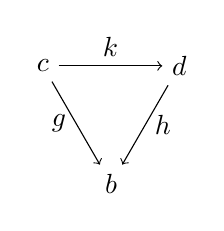
\begin{tikzpicture}
        \begin{scope}[shift={(+3,0)}]
            \draw (150:1) node(ltl){$c$};
            \draw ( 30:1) node(ltr){$d$};
            \draw (270:1) node(lbm){$b$};

            \draw[->] (ltl) to node[below,left ]{$g$}  (lbm);
            \draw[->] (ltr) to node[below,right]{$h$} (lbm);
            \draw[->] (ltl) to node[above]{$k$} (ltr);
        \end{scope}
    \end{tikzpicture}
\]
the pullback functor $f^{\ast} : \catC / b \to \catC / a$ associated with $f$ takes the objects $g : c \to b, h : d \to b$ of $\catC/b$ (morphisms in $\catC$) completes the pullback squares associated with $f$
\[
    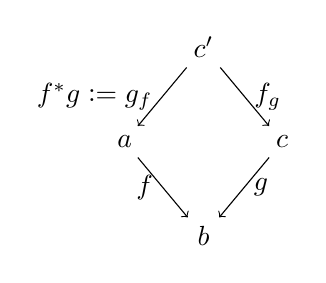
\begin{tikzpicture}
        \begin{scope}[shift={(0,0)}]
            \draw ( 90:1.2) node(t){$c'$};
            \draw (180:1) node(l){$a$};
            \draw (  0:1) node(r){$c$};
            \draw (270:1.2) node(b){$b$};

            \draw[->] (l) to node[below,left ]{$f$} (b);
            \draw[->] (r) to node[below,right]{$g$} (b);
            \draw[->] (t) to node[above,left ]{$f^{\ast}g \vcentcolon= g_{f}$} (l);
            \draw[->] (t) to node[above,right]{$f_{g}$} (r);
        \end{scope}
    \end{tikzpicture}
    \qquad
    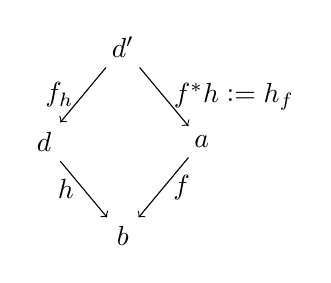
\begin{tikzpicture}
        \begin{scope}[shift={(0,0)}]
            \draw ( 90:1.2) node(t){$d'$};
            \draw (180:1) node(l){$d$};
            \draw (  0:1) node(r){$a$};
            \draw (270:1.2) node(b){$b$};

            \draw[->] (l) to node[below,left ]{$h$} (b);
            \draw[->] (r) to node[below,right]{$f$} (b);
            \draw[->] (t) to node[above,left ]{$f_{h}$} (l);
            \draw[->] (t) to node[above,right]{$f^{\ast}h \vcentcolon= h_{f}$} (r);
        \end{scope}
    \end{tikzpicture}
\]
where a subscript notation $g_{f}$ means ``the pullback of $g$ along $f$''. Defining the action of $f^{\ast} : \catC / b \to \catC / a$ on objects to be $f^{\ast}g = g_{f}$ and $f^{\ast}h = h_{f}$, the action on morphisms in $\catC / b$ is defined by composing the pullback squares with the commuting triangle morphism:
\[
    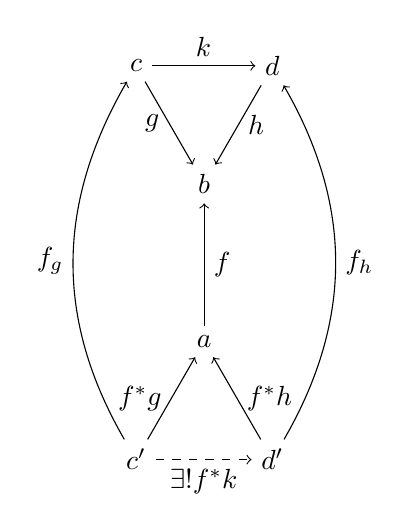
\begin{tikzpicture}
        \begin{scope}[shift={(0,+2)}]
            \draw (150:1) node(t1){$c$};
            \draw ( 30:1) node(t2){$d$};
            \draw (270:1) node(t3){$b$};

            \draw[->] (t1) to node[below,left ]{$g$}  (t3);
            \draw[->] (t2) to node[below,right]{$h$} (t3);
            \draw[->] (t1) to node[above]{$k$} (t2);
        \end{scope}

        \begin{scope}[shift={(0,-2)}]
            \draw (210:1) node(b1){$c'$};
            \draw (330:1) node(b2){$d'$};
            \draw ( 90:1) node(b3){$a$};

            \draw[->] (b1) to node[below,left ]{$f^{\ast}g$} (b3);
            \draw[->] (b2) to node[below,right]{$f^{\ast}h$} (b3);
            \draw[dashed, ->] (b1) to node[below]{$\exists! f^{\ast}k$} (b2);
        \end{scope}
        \draw[->] (b1) to[out=+120, in=-120] node[left ]{$f_{g}$} (t1);
        \draw[->] (b2) to[out=+ 60, in=- 60] node[right]{$f_{h}$} (t2);
        \draw[->] (b3) to node[right]{$f$} (t3);
    \end{tikzpicture}
\]
The commuting triangle in $\catC / a$ appearing at the bottom is completed by a unique morphism \textcolor{red!50!black}{[TODO: why does this morphism need to be unique and exist?]} denoted to be $f^{\ast}k$ ($\neq k_{f}$ obviously). The functoriality of $f^{\ast}$ has a simple proof found here \url{https://proofwiki.org/wiki/Pullback_Functor_is_Functor}.

\subsection{Functors of Monoidal Categories}

\textcolor{red!50!black}{[TODO]}

\subsection{Frobenius Reciprocity}

\textcolor{red!50!black}{[TODO]}



\printbibliography
\end{document}
